\chapter{Application of cohomology}
\label{ch:application_of_cohomology}
In this final chapter on topology, I'll state (mostly without proof)
some nice properties of cohomology groups, and in particular
introduce the so-called cup product.
For an actual treatise on the cup product,
see \cite{ref:hatcher} or \cite{ref:maxim752}.

As mentioned in the previous chapter, you can put all the cohomology groups $H^\bullet(X)$ together
to form the \emph{cohomology ring}, which gives more structure than the case of homology ---
enough structure to allow distinguishing between $\CP^2$ and $S^2 \vee S^4$,
or between $\CP^3$ and $S^2 \times S^4$.

Even though the description above is completely non-descriptive (it doesn't give you insight into
\emph{what} the structure is about), and actually, some people would say:
% https://math.stackexchange.com/q/40149
\begin{quote}
	It does not matter what homology measures intuitively, as it is a convenient tool that takes
	something very difficult (topology) and turns it into something simple (abelian group).
\end{quote}
Nevertheless, it is interesting that the cup product \emph{is actually visualizable}!
At least when the dimension does not exceed $3$.

\section{Poincar\'e duality}
First cool result:
you may have noticed symmetry in the (co)homology groups of
``nice'' spaces like the torus or $S^n$.
In fact this is predicted by:
\begin{theorem}
	[Poincar\'e duality]
	If $M$ is a smooth oriented compact $n$-manifold,
	then we have a natural isomorphism
	\[ H^k(M; \ZZ) \cong H_{n-k}(M) \]
	for every $k$.
	In particular, $H^k(M) = 0$ for $k > n$.
\end{theorem}
So for smooth oriented compact manifolds,
cohomology and homology groups are not so different.

From this follows the symmetry that we mentioned
when we first defined the Betti numbers:
\begin{corollary}
	[Symmetry of Betti numbers]
	Let $M$ be a smooth oriented compact $n$-manifold,
	and let $b_k$ denote its Betti number.
	Then \[ b_k = b_{n-k}. \]
\end{corollary}
\begin{proof}
	\Cref{prob:betti}.
\end{proof}


\section{de Rham cohomology}
\label{sec:de_rham_cohom}
We now reveal the connection between
differential forms and singular cohomology.

Let $M$ be a smooth manifold.
We are interested in the homology and cohomology groups of $M$.
We specialize to the case $G = \RR$, the additive group of real numbers.
\begin{ques}
	Check that $\Ext(H, \RR) = 0$ for any finitely generated abelian group $H$.
\end{ques}
Thus, with real coefficients the universal coefficient theorem says that
\[ H^k(M; \RR) \cong \Hom(H_k(M), \RR) = \left( H_k(M) \right)^\vee \]
where we view $H_k(X)$ as a real vector space.
So, we'd like to get a handle on either $H_k(M$) or $H^k(M; \RR)$.

Consider the cochain complex
\[
	0 \to \Omega^0(M)
	\taking d \Omega^1(M)
	\taking d \Omega^2(M)
	\taking d \Omega^3(M)
	\taking d \dots
\]
and let $\HdR^k(M)$ denote its cohomology groups.
Thus the de Rham cohomology is the closed forms modulo the exact forms.
\[
	\text{Cochain} : \text{Cocycle} : \text{Coboundary}
	= \text{$k$-form} : \text{Closed form} : \text{Exact form}.
\]

The whole punch line is:
\begin{theorem}
	[de Rham's theorem]
	For any smooth manifold $M$, we have a natural isomorphism
	\[ H^k(M; \RR) \cong \HdR^k(M). \]
\end{theorem}
So the theorem is that the real cohomology groups of manifolds $M$
are actually just given by the behavior of differential forms.
Thus,
\begin{moral}
	One can metaphorically think of elements of cohomology groups
	as $G$-valued differential forms on the space.
\end{moral}

Why does this happen?
In fact, we observed already behavior of differential
forms which reflects holes in the space.
For example, let $M = S^1$ be a circle
and consider the \textbf{angle form} $\alpha$
(see \Cref{ex:angle_form}).
The form $\alpha$ is closed, but not exact,
because it is possible to run a full circle around $S^1$.
So the failure of $\alpha$ to be exact is signaling
that $H_1(S^1) \cong \ZZ$.

As another piece of intuition, note that:
\begin{itemize}
	\ii each $k$-differential form $\omega$ can be interpreted as a function that takes each
	$k$-smooth submanifold $S \subseteq M$, and returns a real number $\int_S \omega$.
	\ii let us pretend that all $k$-simplices are smooth for now. Then we have:
	\begin{itemize}
		\ii The $k$-cochains are the functions that sends each $k$-simplex to a real number.
		\ii The $k$-cocycles are the $k$-cochains that sends the boundaries to $0$.
		\ii The $k$-coboundaries are the $k$-cochains that sends the cycles to $0$.
	\end{itemize}

	Meanwhile:
	\begin{itemize}
		\ii The differential forms are the functions that sends each $k$-simplex to a real number,
		satisfying certain linearity and smoothness properties --- for instance:
		\begin{itemize}
			\ii if $k \geq 1$ and a $k$-simplex has the image contained in a point, then it must be
			sent to $0$;
			\ii if we reparametrize a $k$-simplex, the assigned value must be the same;
			\ii if we flip two vertices of a $k$-simplex, the assigned value must be negated;
			\ii if a $k$-simplex can be formed by gluing two $k$-simplices along a face,
			then the assigned value must be the sum of the corresponding values assigned to the
			sub-$k$-simplices;
			\ii etc.
		\end{itemize}
		\ii The closed forms are the differential forms that sends the boundaries to $0$;
		\ii The exact forms are the differential forms that send the cycles to $0$.
	\end{itemize}

	We can't help but noticing the parallel --- the point is:
	\[
		H^k(M; \RR) = \frac{\text{cocycles}}{\text{coboundaries}} \cong
		\frac{\text{cocycles} \cap \text{differential forms}}{\text{coboundaries} \cap
		\text{differential forms}} = \HdR^k(M).
	\]
	Roughly speaking, both the numerator and the denominator on the left are bigger, and they
	\emph{cancels out}.
	We can compare this with \Cref{sec:homology_group_equal}.

	Or, as a figure (for space reasons, the group of differential forms is denoted $D$):
	\begin{center}
	\begin{tikzcd}[column sep=tiny]
		D
			& & \text{cocycles} \\
			& \text{cocycles} \cap D \ar[ul] \ar[ur]
			& & \text{coboundaries} \ar[ul] \\
			& & \text{coboundaries} \cap D \ar[ul] \ar[ur]
	\end{tikzcd}
	\end{center}
	This is precisely the setup of the second isomorphism theorem,%
	\footnote{See \Cref{sec:first_isomorphism_thm}.}
	and you can try to work out why the two quotients are isomorphic.
\end{itemize}

\section{Graded rings}
\prototype{Polynomial rings are commutative graded rings,
while $\Lambda^\bullet(V)$ is anticommutative.}
In the de Rham cohomology, the differential forms can interact in another way:
given a $k$-form $\alpha$ and an $\ell$-form $\beta$, we can consider
a $(k+\ell)$-form
\[ \alpha \wedge \beta. \]
So we can equip the set of forms with a ``product'', satisfying
$\beta \wedge \alpha = (-1)^{k\ell} \alpha \wedge \beta$.
This is a special case of a more general structure:

\begin{definition}
	A \vocab{graded pseudo-ring} $R$ is an abelian group
	\[ R = \bigoplus_{d \ge 0} R^d \]
	where $R^0$, $R^1$, \dots, are abelian groups,
	with an additional associative binary operation $\times \colon R \to R$.
	We require that if $r \in R^d$ and $s \in R^e$, we have $rs \in R^{d+e}$.
	Elements of an $R^d$ are called \vocab{homogeneous elements};
	if $r \in R^d$ and $r \neq 0$, we write $|r| = d$.
\end{definition}
Note that we do \emph{not} assume commutativity.
In fact, these ``rings'' may not even have an identity $1$.
We use other words if there are additional properties:
\begin{definition}
	\label{def:graded_ring}
	A \vocab{graded ring} is a graded pseudo-ring with $1$.
	If it is commutative we say it is a \vocab{commutative graded ring}.
\end{definition}
\begin{definition}
	A graded (pseudo-)ring $R$ is \vocab{anticommutative} if
	for any homogeneous $r$ and $s$ we have
	\[ rs = (-1)^{|r| |s|} sr. \]
\end{definition}

\begin{remark}
	Why not $rs = -sr$? This definition is inspired by the fact that the wedge product is
	anticommutative. Note that, for $f_1, \dots, f_r, g_1, \dots, g_s$ being $0$-forms,
	let $f = df_1 \wedge df_2 \wedge \dots \wedge df_r$ be a $r$-form and
	$g = dg_1 \wedge dg_2 \wedge \dots \wedge dg_s$ be a $s$-form,
	then starting from the expression
	\[ f \wedge g = (df_1 \wedge df_2 \wedge \dots \wedge df_r) \wedge
	(dg_1 \wedge dg_2 \wedge \dots \wedge dg_s) \]
	if you repeatedly swap two adjacent entries, it will take $rs$ swaps total in order to obtain
	the expression
	\[ g \wedge f = (dg_1 \wedge dg_2 \wedge \dots \wedge dg_s) \wedge
	(df_1 \wedge df_2 \wedge \dots \wedge df_r). \]
	By linearity, we can prove that in general, for any $r$-form $f$ and any $s$-form $g$,
	we have $fg = (-1)^{rs} gf$.
\end{remark}
% TODO too clumsy? Also this must have been proven somewhere before?

To summarize:
\begin{center}
	\small
	\begin{tabular}[h]{|c|cc|}
		\hline
		\textbf{Flavors of graded rings} &
		Need not have $1$ & Must have a $1$ \\ \hline
		No Assumption & graded pseudo-ring & graded ring \\
		Anticommutative & anticommutative pseudo-ring & anticommutative ring \\
		Commutative &  & commutative graded ring \\ \hline
	\end{tabular}
\end{center}

\begin{example}[Examples of graded rings]
	\listhack
	\begin{enumerate}[(a)]
		\ii The ring $R = \ZZ[x]$ is a \textbf{commutative graded ring},
		with the $d$th component being the multiples of $x^d$.
		\ii The ring $R = \ZZ[x,y,z]$ is a \textbf{commutative graded ring},
		with the $d$th component being the abelian group
		of homogeneous degree $d$ polynomials (and $0$).
		\ii Let $V$ be a vector space, and consider
		the abelian group
		\[ \Lambda^\bullet(V) = \bigoplus_{d \ge 0} \Lambda^d(V). \]
		For example, $e_1 + (e_2 \wedge e_3) \in \Lambda^\bullet(V)$, say.
		We endow $\Lambda^\bullet(V)$ with the product $\wedge$,
		which makes it into an \textbf{anticommutative ring}.
		\ii Consider the set of differential forms of a manifold $M$,
		say \[ \Omega^\bullet(M) = \bigoplus_{d \ge 0} \Omega^d(M) \]
		endowed with the product $\wedge$.
		This is an \textbf{anticommutative ring}.
	\end{enumerate}
	All four examples have a multiplicative identity.
\end{example}

Let's return to the situation of $\Omega^\bullet(M)$.
Consider again the de Rham cohomology groups $\HdR^k(M)$,
whose elements are closed forms modulo exact forms.
We claim that:
\begin{lemma}
	[Wedge product respects de Rham cohomology]
	The wedge product induces a map
	\[ \wedge \colon \HdR^k(M) \times \HdR^\ell(M) \to \HdR^{k+\ell}(M). \]
\end{lemma}
\begin{proof}
	First, we recall that the operator $d$ satisfies
	\[
		d(\alpha \wedge \beta)
		= (d\alpha) \wedge \beta + \alpha \wedge (d\beta).
	\]
	Now suppose $\alpha$ and $\beta$ are closed forms.
	Then from the above, $\alpha \wedge \beta$ is clearly closed.
	Also if $\alpha$ is closed and $\beta = d\omega$ is exact,
	then $\alpha \wedge \beta$ is exact, from the identity
	\[ d(\alpha \wedge \omega)
		= d\alpha \wedge\omega + \alpha \wedge d\omega = \alpha \wedge \beta. \]
	Similarly if $\alpha$ is exact and $\beta$ is closed
	then $\alpha \wedge \beta$ is exact.
	Thus it makes sense to take the product modulo exact forms,
	giving the theorem above.
\end{proof}

Therefore, we can obtain a \emph{anticommutative ring}
\[ \HdR^\bullet(M) = \bigoplus_{k \ge 0} \HdR^k(M) \]
with $\wedge$ as a product, and $1 \in \Lambda^0(\RR) = \RR$ as the identity.

\section{Cup products}
Inspired by this, we want to see if we can construct a similar product
on $\bigoplus_{k \ge 0} H^k(X; R)$ for any topological space $X$ and ring $R$
(where $R$ is commutative with $1$ as always).
The way to do this is via the \emph{cup product}.

Then this gives us a way to multiply two cochains, as follows.
\begin{definition}
	Suppose $\phi \in C^k(X;R)$ and $\psi \in C^\ell(X;R)$.
	Then we can define their \vocab{cup product}
	$\phi\smile\psi \in C^{k+\ell}(X;R)$ to be
	\[
		(\phi\smile\psi)([v_0, \dots, v_{k+\ell}])
		=
		\phi\left( [v_0, \dots, v_k] \right)
		\cdot
		\psi\left( [v_k, \dots, v_{k+\ell}] \right)
	\]
	where the multiplication is in $R$.
\end{definition}

\begin{ques}
	Assuming $R$ has a $1$, which $0$-cochain is the identity for $\smile$?
\end{ques}

\begin{remark}[Warning]
	While you can interpret a $n$-differential form as a $n$-cochain the obvious way,
	the cup product is \emph{not} directly a generalization of the wedge product!
	For example, let $X = \RR^2$, and try to evaluate $dx \smile dy$ on $[v_0, v_1, v_2]$
	and $[v_2, v_1, v_0]$ where $v_0 = (1, 0)$, $v_1 = (0, 0)$, $v_2 = (0, 1)$,
	assume all of the edges are straight lines.

	This is because we are not having the alternation operator.
	Refer to \Cref{sec:wedge_product_dual} for details.
	In this case, the ring $G$ might be $\ZZ$ where not all nonzero elements have an inverse,
	so division would cause trouble.

	Nevertheless, the differences will nicely cancel out, and
	we still have the corresponding element in the cohomology group equal to
	the element interpreted by the wedge product $dx \wedge dy$ ---
	this is what we mean by $H^\bullet(M; \RR) \cong \HdR^\bullet(M)$, stated below.

	Let us consider the familiar example of a torus, and the $1$-cocycles ``$dx$'' and ``$dy$''.
	\begin{center}
	\begin{asy}
		fill(scale(2)*unitsquare, orange+opacity(0.2));
		draw((0, 0)--(0, 2), blue, MidArrow);
		draw((2, 0)--(2, 2), blue, MidArrow);
		draw((0, 0)--(2, 0), red, MidArrow, L=Label("$dx$", black));
		draw((0, 2)--(2, 2), red, MidArrow);

		draw((0, 0.3)--(1, 0.7), Arrow, L="$\frac{1}{2}$");
		draw((0, 1.1){dir(20)}..(2, 1.1), Arrow, L="$1$");
		draw((0.5, 1.3){dir(70)}..(0.5, 1.9), Arrow, L="$0$");

		fill(shift(3, 0)*scale(2)*unitsquare, orange+opacity(0.2));
		draw((3, 0)--(3, 2), blue, MidArrow);
		draw((5, 0)--(5, 2), blue, MidArrow);
		draw((3, 0)--(5, 0), red, MidArrow, L=Label("$dy$", black));
		draw((3, 2)--(5, 2), red, MidArrow);

		draw((3, 1.1){dir(20)}..(5, 1.1), Arrow, L="$0$");
		draw((4.2, 0){dir(70)}..(4.2, 2), Arrow, L="$1$");
	\end{asy}
	\end{center}

	From what we know about the wedge product, we want $(dx \wedge dy)(T) = 1$ for $T$ the whole
	torus (up to a $\pm$ sign). Indeed, with the definition above (work it out! Divide $T$ into two
	triangles arbitrarily) it will work.

	Nevertheless, we don't really care about the cup product itself as much as the induced cup
	product on the homology ring.
\end{remark}

First, we prove an analogous result as before:
\begin{lemma}[$\delta$ with cup products]
	We have
	$\delta(\phi\smile\psi) = \delta\phi\smile\psi
	+ (-1)^k\phi\smile\delta\psi$.
\end{lemma}
\begin{proof}
	Direct $\sum$ computations.
\end{proof}
Thus, by the same routine we used for de Rham cohomology, we get
an induced map
\[ \smile \colon H^k(X;R) \times H^\ell(X;R) \to H^{k+\ell}(X;R).  \]
We then define the \vocab{singular cohomology ring}
whose elements are finite sums in
\[ H^\bullet(X;R) = \bigoplus_{k \ge 0} H^k(X;R) \]
and with multiplication given by $\smile$.
Thus it is a graded ring (with $1_R \in R$ the identity)
and is in fact anticommutative:
\begin{proposition}[Cohomology is anticommutative]
	$H^\bullet(X; R)$ is an anticommutative ring,
	meaning $\phi \smile \psi = (-1)^{k\ell} \psi \smile \phi$.
\end{proposition}
For a proof, see \cite[Theorem 3.11, pages 210-212]{ref:hatcher}.
Moreover, we have the de Rham isomorphism
\begin{theorem}
	[de Rham extends to ring isomorphism]
	For any smooth manifold $M$, the isomorphism
	of de Rham cohomology groups to singular cohomology
	groups in facts gives an isomorphism
	\[ H^\bullet(M; \RR) \cong \HdR^\bullet(M) \]
	of anticommutative rings.
\end{theorem}

Therefore, if ``differential forms'' are the way to visualize
the elements of a cohomology group, the wedge product is the
correct way to visualize the cup product.

We now present (mostly without proof)
the cohomology rings of some common spaces.

\begin{example}
	[Cohomology of torus]
	The cohomology ring $H^\bullet(S^1 \times S^1; \ZZ)$
	of the torus is generated by elements $|\alpha| = |\beta| = 1$
	which satisfy the relations
	$\alpha \smile \alpha = \beta \smile \beta = 0$,
	and $\alpha \smile \beta = -\beta \smile \alpha$.
	(It also includes an identity $1$.)
	Thus as a $\ZZ$-module it is
	\[ H^\bullet(S^1 \times S^1; \ZZ)
		\cong \ZZ \oplus \left[ \alpha \ZZ \oplus \beta \ZZ \right]
		\oplus (\alpha \smile \beta) \ZZ. \]
	This gives the expected dimensions $1+2+1=4$.
	It is anti-commutative.
\end{example}

You have already seen the elements $\alpha$ and $\beta$ as the elements called $dx$ and $dy$ in the
remark above.

\begin{example}[Cohomology ring of $S^n$]
	Consider $S^n$ for $n \ge 1$.
	The nontrivial cohomology groups are given by
	$H^0(S^n; \ZZ) \cong H^n(S^n; \ZZ) \cong \ZZ$.
	So as an abelian group
	\[ H^\bullet(S^n; \ZZ) \cong \ZZ \oplus \alpha \ZZ \]
	where $\alpha$ is the generator of $H^n(S^n, \ZZ)$.

	Now, observe that $|\alpha\smile\alpha| = 2n$, but
	since $H^{2n}(S^n; \ZZ) = 0$ we must have $\alpha\smile\alpha=0$.
	So even more succinctly,
	\[ H^\bullet(S^n; \ZZ) \cong \ZZ[\alpha]/(\alpha^2). \]
	Confusingly enough, this graded ring is both
	commutative \emph{and} anti-commutative.
	The reason is that $\alpha \smile \alpha = 0 = -(\alpha \smile \alpha)$.
\end{example}

\begin{example}[Cohomology ring of real and complex projective space]
	It turns out that
	\begin{align*}
		H^\bullet(\RP^n; \Zc2) &\cong \Zc2[\alpha]/(\alpha^{n+1}) \\
		H^\bullet(\CP^n; \ZZ) &\cong \ZZ[\beta]/(\beta^{n+1})
	\end{align*}
	where $|\alpha| = 1$ is a generator of $H^1(\RP^n; \Zc2)$
	and $|\beta| = 2$ is a generator of $H^2(\CP^n; \ZZ)$.

	Confusingly enough, both graded rings are commutative \emph{and} anti-commutative.
	In the first case it is because we work in $\Zc 2$, for which $1 = -1$,
	so anticommutative is actually equivalent to commutative.
	In the second case, all nonzero homogeneous elements have degree $2$.
\end{example}

Already we have an interesting example where the cup product $\smile$ is different from the
wedge product $\wedge$ --- if $n \geq 2$, then the generators $\alpha$ and $\beta$ above has
$\alpha \smile \alpha \neq 0$ and $\beta \smile \beta \neq 0$.

Let us try to see what happens here. The formula above says
\[ H^\bullet(\RP^2; \Zc2) \cong \Zc2[\alpha]/(\alpha^3) \]
As an abelian group, there is a single nonzero element in
$H^0(\RP^2; \Zc2)$, $H^1(\RP^2; \Zc2)$, and $H^2(\RP^2; \Zc2)$,
and the remaining groups are $0$.

$\RP^2$ isn't too hard to visualize --- it's just a $2$-sphere, quotient by the relation to identify
opposite vertices.

There is a $1$-cycle on it that is not homologous to $0$:
\begin{center}
	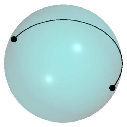
\includegraphics{3dfigures/pdf/1cycle.pdf}
\end{center}
It's not very easy to show, but every such $1$-cycle is homologous to each other,
and double of that cycle is homologous to $0$.

As such, $H^1(\RP^2; \Zc2) \cong \Hom(H_1(\RP^2), \Zc2)$, its only nontrivial element $\alpha$
maps each such $1$-cycle to $1$.

\begin{center}
\begin{asy}
	size(3cm);
	fill(scale(2)*unitsquare, orange+opacity(0.2));
	draw((0, 0)--(0, 2), blue, MidArrow);
	draw((2, 2)--(2, 0), blue, MidArrow);
	draw((0, 0)--(2, 0), red, MidArrow);
	draw((2, 2)--(0, 2), red, MidArrow);
	label("$a$", (0, 2), NW);
	label("$b$", (2, 2), NE);
	label("$c$", (0, 0), SW);
	label("$d$", (2, 0), SE);
	draw((0.5, 0)--(0.5, 2), Arrow);
\end{asy}
\end{center}

Consider $\alpha \smile \alpha$. Notice that $\alpha$ acts like both $dx$ and $dy$ at the same time
(both the blue edge and the red edge got assigned the value $1$), so it assigns the value $1$ to the
whole surface of the real projective plane! Thus it's nontrivial.

\begin{exercise}
	Manually compute the cup product $\alpha \smile \alpha$ to verify that.
	(Divide the surface into some triangles. $[a, c, d] + [a, d, b] - [c, c, d] + [c, d, c]$ is a
	working choice. Verify that the boundary is nonzero, but is divisible by $2$.)
\end{exercise}

\section{Relative cohomology pseudo-rings}
For $A \subseteq X$, one can also define a relative cup product
\[ H^k(X,A;R) \times H^\ell(X,A;R) \to H^{k+\ell}(X,A;R). \]
After all, if either cochain vanishes on chains in $A$,
then so does their cup product.
This lets us define \vocab{relative cohomology pseudo-ring}
and \vocab{reduced cohomology pseudo-ring} (by $A = \{\ast\}$), say
\begin{align*}
H^\bullet(X,A;R) &= \bigoplus_{k \ge 0} H^k(X,A; R) \\
\wt H^\bullet(X;R) &= \bigoplus_{k \ge 0} \wt H^k(X;R).
\end{align*}
These are both \textbf{anticommutative pseudo-rings}.
Indeed, often we have $\wt H^0(X;R) = 0$ and thus there is no identity at all.

Once again we have functoriality:
\begin{theorem}
	[Cohomology (pseudo-)rings are functorial]
	Fix a ring $R$ (commutative with $1$).
	Then we have functors
	\begin{align*}
		H^\bullet(-; R) &: \catname{hTop}\op \to \catname{GradedRings} \\
		H^\bullet(-,-; R) &: \catname{hPairTop}\op \to \catname{GradedPseudoRings}.
	\end{align*}
\end{theorem}

Unfortunately, unlike with (co)homology groups,
it is a nontrivial task to determine\footnote{Apart from the method of passing to differential
form and back, that is. You have already computed a wedge product above.} the cup product
for even nice spaces like CW complexes.
So we will not do much in the way of computation.
However, there is a little progress we can make.

\section{Wedge sums}
Our goal is to now compute $\wt H^\bullet(X \vee Y)$.
To do this, we need to define the product of two graded pseudo-rings:
\begin{definition}
	Let $R$ and $S$ be two graded pseudo-rings.
	The \vocab{product pseudo-ring} $R \times S$ is the graded pseudo-ring
	defined by taking the underlying abelian group as
	\[ R \oplus S = \bigoplus_{d \ge 0} (R^d \oplus S^d). \]
	Multiplication comes from $R$ and $S$, followed by
	declaring $r \cdot s = 0$ for $r \in R$, $s \in S$.
\end{definition}
Note that this is just graded version of the product ring
defined in \Cref{ex:product_ring}.
\begin{exercise}
	Show that if $R$ and $S$ are graded rings (meaning they have $1_R$ and $1_S$),
	then so is $R \times S$.
\end{exercise}

Now, the theorem is that:
\begin{theorem}
	[Cohomology pseudo-rings of wedge sums]
	We have
	\[
		\wt H^\bullet(X \vee Y; R)
		\cong \wt H^\bullet(X;R)
		\times \wt H^\bullet(Y;R)
	\]
	as graded pseudo-rings.
\end{theorem}

Knowing just that the rings are isomorphic doesn't help much, it would be much better if you know
what the isomorphism is --- so that in simple cases, you can see for yourself the rings are
isomorphic.

The isomorphism is the most trivial one:
Given $f \in C^\bullet(X \vee Y; R)$ that assigns to each chain $c$ inside $X \vee Y$ a value
$f(c) \in R$, we can interpret it as an element of $C^\bullet(X)$, because each chain inside $X$ is
trivially a chain inside $X \vee Y$ that can be fed into $f$ ---
formally, the embedding $X \injto X \vee Y$ induces
$C_\bullet(X) \injto C_\bullet(X \vee Y)$. The map induces a $\wt H^\bullet(X \vee Y; R)
\to \wt H^\bullet(X; R) \times \wt H^\bullet(Y; R)$, and it respects the ring multiplication i.e.
the cup product.

\begin{example}
	Let $X$ and $Y$ be depicted as in the following figure.
	\begin{center}
	\begin{asy}
		draw(scale(0.5)*shift(1, 1)*unitcircle);
		draw(shift(-1, 0)*unitsquare);
		label("$=$", (1.25, 0.5));
		draw(shift(1.5, 0)*unitsquare);
		label("$\vee$", (2.75, 0.5));
		draw(shift(3, 0)*scale(0.5)*shift(1, 1)*unitcircle);
	\end{asy}
	\end{center}
	Let $f \in \wt H^1(X; \ZZ)$ assigns $f(X) = 2$ to the whole square, and
	$g \in \wt H^1(Y; \ZZ)$ assigns $g(Y) = 3$ to the whole circle.
	Then, of course the element corresponds to $(f, g)$ inside $\wt H^1(X \vee Y)$ would assigns
	$2 + 3 = 5$ to the cocycle corresponding to the whole space $X \vee Y$.
\end{example}

This allows us to resolve the first question posed at the beginning.
Let $X = \CP^2$ and $Y = S^2 \vee S^4$.
We have that
\[ H^\bullet(\CP^2; \ZZ) \cong \ZZ[\alpha] / (\alpha^3). \]
Hence this is a graded ring generated by there elements:
\begin{itemize}
	\ii $1$, in dimension $0$.
	\ii $\alpha$, in dimension $2$.
	\ii $\alpha^2$, in dimension $4$.
\end{itemize}
Next, consider the reduced cohomology pseudo-ring
\[ \wt H^\bullet(S^2 \vee S^4; \ZZ) \cong
	\wt H^\bullet(S^2; \ZZ)
	\oplus \wt H^\bullet(S^4 ; \ZZ).
\]
Thus the absolute cohomology ring $H^\bullet(S^2 \vee S^4 ; \ZZ)$
is a graded ring also generated by three elements.
\begin{itemize}
	\ii $1$, in dimension $0$ (once we add back in the $0$th dimension).
	\ii $a_2$, in dimension $2$ (from $H^\bullet(S^2 ; \ZZ)$).
	\ii $a_4$, in dimension $4$ (from $H^\bullet(S^4 ; \ZZ)$).
\end{itemize}
Each graded component is isomorphic, like we expected.
However, in the former, the product of two degree $2$ generators is
\[ \alpha \cdot \alpha = \alpha^2. \]
In the latter, the product of two degree $2$ generators is
\[ a_2 \cdot a_2 = a_2^2 = 0 \]
since $a_2 \smile a_2 = 0 \in H^\bullet(S^2; \ZZ)$.

Thus $S^2 \vee S^4$ and $\CP^2$ are not homotopy equivalent.

Intuitively, what the proof above says is:
\begin{moral}
	The nontrivial $4$-cocycle $a_4 \in H^4(S^2 \vee S^4; \ZZ)$
	has nothing to do with the $2$-cocycle $a_2$,
	while the $4$-cocycle $\alpha^2 \in H^4(\CP^2)$ is the cup product $\alpha
	\smile \alpha$ of the $2$-cocycle $\alpha$ with itself.
\end{moral}

The exercise below would be much easier to visualize, apart from the fact that $\RP^2$ is
nonorientable --- in fact, we have already seen
above why $\alpha \smile \alpha \neq 0$ for the nonzero element $\alpha \in H^1(\RP^2)$.

\begin{exercise}
	Similarly, show that $S^1 \vee S^2$ and $\RP^2$ are not homotopy equivalent by showing
	$\wt H^\bullet(S^1 \vee S^2; \Zc 2) \not\cong \wt H^\bullet(\RP^2; \Zc 2)$,
	even though each graded component is isomorphic.
\end{exercise}

\section{Cross product}

In this section, we will define the cross product.

\subsection{Motivation}

Roughly speaking, the motivation is the following:
\begin{moral}
	If $X$ has a $m$-dimensional hole and $Y$ has a $n$-dimensional hole, then $X \times Y$ has a
	$(m + n$)-dimensional hole.
\end{moral}
Which is true in most common cases under suitable interpretation of ``holes''
(either with homology, or with cohomology).

We will formalize and prove the statement above.

\subsection{Cross product on singular homology}

First, we define the \vocab{cross product}, that takes a $m$-simplex $f \colon \Delta^m \to X$ and a
$n$-simplex $g \colon \Delta^n \to Y$, and returns a $(m + n)$-chain $f \times g \in C_{m + n}(X
\times Y)$.\footnote{As far as I know, this is just because the symbol $\times$ is a cross, and it
has nothing to do with the cross product of vectors in $\RR^3$.}
This is really the most natural way you might define it: intuitively, the product of a
$m$-dimensional cube in $X$ and a $n$-dimensional cube in $Y$ is a $(m + n)$-dimensional cube in $X
\times Y$.
\begin{center}
\begin{asy}
	draw((0.5, 0)--(2.5, 0), L=Label("$X$", EndPoint, align=NE));
	draw((0, 0.5)--(0, 2.5), L=Label("$Y$", EndPoint, align=NE));
	draw((1, 0)--(2, 0), blue+1, L=Label("$U$", EndPoint, align=NE));
	dot((1, 0), blue);
	dot((2, 0), blue);
	draw((0, 1)--(0, 2), blue+1, L=Label("$V$", EndPoint, align=NE));
	dot((0, 1), blue);
	dot((0, 2), blue);
	filldraw(shift(1, 1)*unitsquare, blue+opacity(0.1), blue);
	label("$U \times V$", (2, 2), blue, align=N);
	draw(shift(0.5, 0.5)*scale(2)*unitsquare);
	label("$X \times Y$", (2.5, 2.5), align=N);
\end{asy}
\end{center}

In the case of a simplex, we need to subdivide $\Delta^m \times \Delta^n$ into finitely many copies
of $\Delta^{m + n}$.

If $n = 1$, we have already seen a subdivision when we worked with the prism operator. For the
general case, refer to \cite[page 277]{ref:hatcher} --- the number blows up quickly, for example,
you need $\binom{30}{15}=155117520$ simplices to cover $\Delta^{15} \times \Delta^{15}$!

Formally, we can define the cross product of chains: that is, a function
\[ C_m(X) \times C_n(Y) \taking\times C_{m \times n}(X \times Y). \]
We can prove that this induces a map on homology groups:
\[ H_m(X) \times H_n(Y) \taking\times H_{m \times n}(X \times Y). \]

\begin{exercise}
	Let $X = Y = S^1$, so that $X \times Y$ is a torus.
	Let $\alpha$ be a generator of $H_1(X)$, and $\beta$ be a generator of $H_1(Y)$.
	Show that $\alpha \times \beta$ is the generator of $H_2(X \times Y)$.
\end{exercise}

Actually, we have the following:
\begin{theorem}
	\label{thm:topological_kunneth_1}
	% theorem 3B.6 in Hatcher, specialized
If $X$ and $Y$ are CW complexes and $R$ is a PID, then the cross product of two nonzero elements in
$H_m(X)$ and $H_n(Y)$ is nonzero.
\end{theorem}

Thus formalize our intuition earlier --- at least, if we use homology as a measure of ``holes''.

\subsection{Cross product is not a $\ZZ$-module homomorphism}

For this section, if $a$ and $b$ are elements of the $\ZZ$-module $C_m(X)$ and $C_n(Y)$ respectively,
we write $\times(a, b)$ to mean $a \times b \in C_{m + n}(X \times Y)$, and $(a, b)$
to be the element that corresponds in the product $C_m(X) \times C_n(Y)$.

There is a little technical detail that we need to sort out --- above, we writes
\[ \times \colon C_m(X) \times C_n(Y) \to C_{m + n}(X \times Y). \]
But written this way, $\times$ is not a $\ZZ$-module homomorphism!

\begin{example}
	Let $a$ and $b$ be any nonzero elements in $C_m(X)$ and $C_n(Y)$ respectively.

	Then,
	\begin{align*}
		\times(a, b) &= a \times b \\
		2 \cdot (a, b) &= (2a, 2b) \\
		\times(2 \cdot (a, b)) &= 4(a \times b).
	\end{align*}
\end{example}

If we want to talk about isomorphism, or do anything with the $\ZZ$-module structure of $C_{m + n}(X
\times Y)$ or $H_{m + n}(X \times Y)$, we'd better having a $\ZZ$-module homomorphism.

This is easy enough to fix: $\times$ is bilinear, so it's natural to consider the tensor product:
\[ \times \colon C_m(X) \otimes_\ZZ C_n(Y) \to C_{m + n}(X \times Y). \]
With this notation, $\times(a \otimes b) = a \times b$.
(As a side effect, we can also write
$\times(a \otimes b + c \otimes d) = a \times b + c \times d$ now.)

And so, let us restate \Cref{thm:topological_kunneth_1}:
\begin{theorem}
	If $X$ and $Y$ are CW complexes, then
	\[ \times \colon H_m(X) \otimes_\ZZ H_n(Y) \to H_{m + n}(X \times Y) \]
	is an injective $\ZZ$-module homomorphism.
\end{theorem}

\subsection{Cross product on cellular homology}

The definition with singular homology is quite clumsy ---
because we use simplices as the building blocks for the chains,
the product of two simplices in $X$ and $Y$ becomes a huge collection of simplices in $X \times Y$.

We will now redefine the cross product using cellular homology ---
it can be safely skipped, since both definitions of the cross product gives identical result on the
homology groups.

If $X$ and $Y$ are CW complexes, we can do better.
We see that $X \times Y$ has a natural CW complex structure: for each cell $e^m$ of $X$ and cell
$e^n$ of $Y$, their product makes for a cell $e^{m + n}$ of $X \times Y$.

\begin{example}
	If $X$ and $Y$ are both line segments built from
	two $0$-cells and one $1$-cell, then their product $X \times Y$ has a natural CW complex
	structure containing:
	\begin{itemize}
		\ii $4$ $0$-cells,
		\ii $4$ $1$-cells,
		\ii $1$ $2$-cell.
	\end{itemize}
\end{example}

Recall the cellular groups $\Cells_\bullet(X)$ from \Cref{ch:cellular_homology}, each basis element
corresponds to a cell in $X$.
Then, we can define the cross product on the basis elements:
\[ \times \colon \Cells_m(X) \otimes_\ZZ \Cells_n(Y) \to \Cells_{m + n}(X \times Y). \]
To be painfully explicit:
let $e^m \in \Cells_m(X)$, $e^n \in \Cells_m(Y)$, then the cross product is defined by $e^m \times
e^n = e^m \times e^n \in \Cells_{m + n}(X \times Y)$ --- even the notation used is trivial.

Of course, this induces a map on the homology groups:
\[ \times \colon H_m(X) \otimes_\ZZ H_n(Y) \to H_{m + n}(X \times Y). \]
This map is the same as the map we defined earlier.

\subsection{Cross product on cellular cohomology}

We do the same thing as above, but this time with cohomology --- remember that homology and
cohomology are slightly different measures of ``holes'', for $K$ the Klein bottle then $H_2(X) =
0$ but $H^2(X; \ZZ) \neq 0$.

Given two cellular cochains $f \in \Hom(\Cells_m(X); R)$ and
$g \in \Hom(\Cells_n(Y); R)$, we want to obtain a cochain $f
\times g \in \Hom(\Cells_{m + n}(X \times Y); R)$.

Of course, it is defined in the most natural way possible: for a cell $e^m$ of $X$ and a cell $e^n$
of $Y$, we have $(f \times g)(e^m \times e^n) = f(e^m) \cdot g(e^n)$.

Sounds good? Not yet --- since not all $(m + n)$-cells $e^{m + n}$ of $X \times Y$
is formed as a product of a $m$-cell in $X$ and a $n$-cell in $Y$.
For those, we simply declare that $(f \times g)(e^{m + n}) = 0$.

As usual, this map induces a $R$-module homomorphism on the cohomology groups:
\[ \times \colon H^m(X; R) \otimes_R H^n(Y; R) \to H^{m + n}(X \times Y; R). \]

\subsection{Motivation: cross product of differential forms}

The definition of the cross product of two cellular cochains above are clean, but may appear to be
dry and unmotivated.

Turns out you can do the same thing on differential form.
What's more, it gives a clean way of defining the wedge product $\alpha \wedge \beta$!
Let's see it in action.

Instead of the definition, here are a few examples. Motivated readers may try to define the concept
formally.
\begin{example}[Examples of cross product of differential form]
	Here are a few examples.
	\begin{itemize}
		\ii If $X$ and $Y$ are the $x$-axis and the $y$-axis of the plane respectively,
		the cross product $dx \times 2dy$ is equal to $2(dx \wedge dy)$.

		Certainly this is natural --- as $dx$ assigns the value $1$ to the vector $\ee_1$,
		and $2dy$ assigns the value $2$ to the vector $\ee_2$, we get that $dx \times 2dy$ should
		assigns the value $1 \cdot 2 = 2$ to the unit square spanned by $\ee_1$ and $\ee_2$ --- that
		is, $\ee_1 \wedge \ee_2$.
		\ii Let $X$ be the $xy$-plane, and let $Y$ be the $z$-axis.
		Consider the cross product $dx \times dz$. What $2$-form should the result be?

		Certainly, we should have $(dx \times dz)(\ee_1 \wedge \ee_3) = 1$
		and $(dx \times dz)(\ee_2 \wedge \ee_3) = 0$.
		But this isn't enough to uniquely determines $dx \times dz$.

		And so, we declares: $(dx \times dz)(\ee_1 \wedge \ee_2) = 0$.
		With this, we get $dx \times dz = dx \wedge dz$.
	\end{itemize}
\end{example}

More generally, we can define the cross product by picking a basis for $X$ and $Y$, and define the
value of $\alpha \times \beta$ on the basis elements.

As promised --- you can define the wedge product using the cross product.
There's only one thing you can do:
\begin{definition}[Definition of wedge product using the cross product]
	For $X$ a $\RR$-vector space,
	let $\alpha \in (\Lambda^m(X))^\vee$ and $\beta \in (\Lambda^n(X))^\vee$,
	then $\alpha \wedge \beta \in (\Lambda^{m + n}(X)$ is defined by
	\[
		\alpha \wedge \beta = \Delta^*(\alpha \times \beta)
	\]
	where $\Delta \colon X \to X \times X$, $\Delta(x) = (x, x)$ is the diagonal map.
	Recall that $\Delta^*$ denotes the pullback operation.
\end{definition}
In simpler terms:
to evaluate $\alpha \wedge \beta$ on a $(m + n)$-wedge in $X$,
push it to $X \times X$ using the diagonal map, and give it to $\alpha \times \beta$.

\subsection{Piecing the cohomology groups together}

Recall that we have above the $R$-module homomorphism
\[ \times \colon H^m(X; R) \otimes_R H^n(Y; R) \to H^{m + n}(X \times Y; R). \]
We know that it is in fact possible to piece all the $H^\bullet(X; R)$ together to form
an anticommutative graded ring, the cohomology ring. So we wish to extend the map to a
$R$-algebra homomorphism
\[ \times \colon H^\bullet(X; R) \otimes_R H^\bullet(Y; R) \to H^\bullet(X \times Y; R). \]

We haven't defined what the tensor product of two graded rings is yet --- we will formally do that
in the next section, but intuitively, it consists of all the $H^m(X; R) \otimes_R H^n(Y; R)$
pieced together.

\section{K\"unneth formula}
We now wish to tell apart the spaces $S^2 \times S^4$ and $\CP^3$.
In order to do this, we will need a formula
for $H^n(X \times Y; R)$ in terms of $H^n(X;R)$ and $H^n(Y;R)$.
These formulas are called \vocab{K\"unneth formulas}.
In this section we will only use a very special case,
which involves the tensor product of two graded rings.

\begin{definition}
	Let $A$ and $B$ be two graded rings which are also $R$-modules
	(where $R$ is a commutative ring with $1$).
	We define the \vocab{tensor product} $A \otimes_R B$ as follows.
	As an abelian group, it is
	\[ A \otimes_R B = \bigoplus_{d \ge 0}
		\left( \bigoplus_{k=0}^{d} A^k \otimes_R B^{d-k}  \right). \]
	The multiplication is given on basis elements by
	\[ \left( a_1 \otimes b_1 \right)\left( a_2 \otimes b_2 \right)
		= (a_1a_2) \otimes (b_1b_2).
	\]
	Of course the multiplicative identity is $1_A \otimes 1_B$.
\end{definition}

Now let $X$ and $Y$ be topological spaces, and take the product:
we have a diagram
\begin{center}
\begin{tikzcd}
	& X \times Y \ar[ld, "\pi_X"'] \ar[rd, "\pi_Y"] \\
	X && Y
\end{tikzcd}
\end{center}
where $\pi_X$ and $\pi_Y$ are projections.
As $H^k(-; R)$ is functorial, this gives induced maps
\begin{align*}
	\pi_X^\ast &: H^k(X \times Y; R) \to H^k(X; R) \\
	\pi_Y^\ast &: H^k(X \times Y; R) \to H^k(Y; R)
\end{align*}
for every $k$.

By using this, we can define a so-called cross product.
\begin{definition}
	Let $R$ be a ring, and $X$ and $Y$ spaces.
	Let $\pi_X$ and $\pi_Y$ be the projections of $X \times Y$
	onto $X$ and $Y$.
	Then the \vocab{cross product} is the map
	\[
		H^\bullet(X; R) \otimes_R H^\bullet(Y;R)
		\taking{\times} H^\bullet(X \times Y; R)
	\]
	acting on cocycles as follows:
	$\phi \times \psi = \pi_X^\ast(\phi) \smile \pi_Y^\ast(\psi)$.
\end{definition}

This is just the most natural way to take a $k$-cocycle
on $X$ and an $\ell$-cocycle on $Y$, and create a $(k+\ell)$-cocycle
on the product space $X \times Y$.

\begin{remark}
	Of course, this definition coincides with the definition above using cellular cohomology, but
	the proof is omitted.
\end{remark}

\begin{theorem}
	[K\"unneth formula]
	% theorem 3.15 in Hatcher
	Let $X$ and $Y$ be CW complexes such that $H^k(Y;R)$
	is a finitely generated free $R$-module for every $k$.
	Then the cross product is an isomorphism of anticommutative rings
	\[
		H^\bullet(X;R) \otimes_R H^\bullet(Y;R)
		\to H^\bullet(X \times Y; R).
	\]
\end{theorem}

That is:
\begin{moral}
	There is a one-to-one correspondence between pair of holes in $X$ and $Y$
	and holes of $X \times Y$.
	Furthermore, the correspondence respects the cup product.
\end{moral}
Where ``holes'' is to be understood as ``generators of cohomology groups'' in this case.

In any case, this finally lets us resolve the question
set out at the beginning.
We saw that $H_n(\CP^3) \cong H_n(S^2 \times S^4)$ for every $n$,
and thus it follows that $H^n(\CP^3; \ZZ) \cong H^n(S^2 \times S^4; \ZZ)$ too.

But now let us look at the cohomology rings. First, we have
\[ H^\bullet(\CP^3; \ZZ) \cong \ZZ[\alpha] / (\alpha^4)
	\cong \ZZ \oplus \alpha\ZZ \oplus \alpha^2\ZZ \oplus \alpha^3\ZZ
\]
where $|\alpha| = 2$; hence this is a graded ring generated by
\begin{itemize}
	\ii $1$, in degree $0$.
	\ii $\alpha$, in degree $2$.
	\ii $\alpha^2$, in degree $4$.
	\ii $\alpha^3$, in degree $6$.
\end{itemize}

Now let's analyze
\[ H^\bullet(S^2 \times S^4; \ZZ) \cong
	\ZZ[\beta] / (\beta^2)
	\otimes
	\ZZ[\gamma] / (\gamma^2).
\]
It is thus generated thus by the following elements:
\begin{itemize}
	\ii $1 \otimes 1$, in degree $0$.
	\ii $\beta \otimes 1$, in degree $2$.
	\ii $1 \otimes \gamma$, in degree $4$.
	\ii $\beta \otimes \gamma$, in degree $6$.
\end{itemize}
Again in each dimension we have the same abelian group.
But notice that if we square $\beta \otimes 1$ we get
\[ (\beta \otimes 1)(\beta \otimes 1) = \beta^2 \otimes 1 = 0. \]
Yet the degree $2$ generator of $H^\bullet(\CP^3; \ZZ)$
does not have this property.
Hence these two graded rings are not isomorphic.

\begin{moral}
	The nontrivial $4$-cocycle $1 \otimes \gamma$ of $S^2 \times S^4$ is orthogonal to the
	$2$-cocycle $\beta \otimes 1$, while the $4$-cocycle $\alpha^2$ of $\CP^3$ is the cup product
	$\alpha \smile \alpha$ of the $2$-cocycle $\alpha$ with itself.
\end{moral}

So it follows that $\CP^3$ and $S^2 \times S^4$ are not homotopy equivalent.

\begin{exercise}
	Do the same procedure with $H^\bullet(\RP^3; \Zc 2)$ and $H^\bullet(S^1 \times S^2; \Zc 2)$.
	(Visualize $S^1 \times S^2$ as a thickened sphere with the outer and inner face fused together,
	and $RP^3$ as a closed $3$-ball with opposing points on the boundary surface fused together.
	Try to stretch your mind and guess what the homology and cohomology groups are before formally
	compute it.)
\end{exercise}

% Borsuk Ulam

\section\problemhead

\begin{dproblem}
	[Symmetry of Betti numbers by Poincar\'e duality]
	\label{prob:betti}
	Let $M$ be a smooth oriented compact $n$-manifold,
	and let $b_k$ denote its Betti number.
	Prove that $b_k = b_{n-k}$.
	\begin{hint}
		Write $H^k(M; \ZZ)$ in terms of $H_k(M)$
		using the UCT, and analyze the ranks.
	\end{hint}
\end{dproblem}

\begin{problem}
	Show that $\RP^n$ is not orientable for even $n$.
	\begin{hint}
		Use the previous result on Betti numbers.
	\end{hint}
\end{problem}

\begin{problem}
	Show that $\RP^3$ is not homotopy equivalent to $\RP^2 \vee S^3$.
	\begin{hint}
		Use the $\Zc2$ cohomologies, and find the cup product.
	\end{hint}
\end{problem}

\begin{problem}
	\gim
	Show that $S^m \vee S^n$ is not a deformation retract
	of $S^m \times S^n$ for any $m,n \ge 1$.
	\begin{hint}
		Assume that $r \colon S^m \times S^n \to S^m \vee S^n$ is such a map.
		Show that the induced map
		$H^\bullet(S^m \vee S^n; \ZZ) \to H^\bullet(S^m \times S^n; \ZZ)$
		between their cohomology rings is monic
		(since there exists an inverse map $i$).
	\end{hint}
	\begin{sol}
		See \cite[Example 3.3.14, pages 68-69]{ref:maxim752}.
	\end{sol}
\end{problem}
